\input{D:/Physics/Program/Book-begin.tex}
%\usepackage{ctex}
\usepackage{multirow}  % 允许单元格合并
\usepackage{booktabs}  % 提供更美观的表格线

\title{\textbf{Documentation for GEONU Software}}
\author{Shuai Ouyang\thanks{\parbox[t]{4.5cm}{%
			\texttt{shuaiouyang@mail.sdu.edu.cn} \\ 
			\texttt{Shuai.Ouyang@snolab.ca}}}}
\date{2025.03.21}

\begin{document}
	\pdfbookmark{Book Cover}{title} 	%创建封面pdf标签;第一个{}参数是pdf标签的名字,第二个{}参数用于hyperlink,
	\maketitle							%显示封面
	\thispagestyle{empty}				%封面取消页码
	\frontmatter						%页码使用罗马字母
	\cleardoublepage				 	%消除一张空白页,为了在pdf中实现目录的跳转
	\pdfbookmark{\contentsname}{toc} 	%创建目录pdf标签
	\tableofcontents				  	%生成目录
	\mainmatter							%页码使用拉丁数
	\chapter{Introduction}
		\section{What is Geoneutrino}
			Geoneutrino is electron antineutrino originating from the interior of the earth, and it was firstly proposed in geological research. With the development of seismology, we have gained a understanding of the Earth's physical structure, but we still know little about its chemical properties. These chemical properties have an important impact on the Earth's evolution, such as continental drift and mantle convection. Although, there are several theories currently describe the Earth's internal chemical composition, experimental validation is needed to determine which theory is correct, since there are no direct measurements of the mantle. Geoneutrino detection is the only method currently available to probe this mystery.\par
			
			Radiogenic power is one of the key energy sources driving Earth's internal dynamics. It it generated by the decay of heat-producing elements (HPEs), such as ${}^{235}$U, $^{238}$U, ${}^{232}$Th and ${}^{40}$K. These elements undergo weak decay processes \cite{fiorentini2007geo} (Eq.\ref{Decay:U235}-\ref{Decay:K40_2}) and emit neutrinos in the process. Due to their extremely weak interaction with matter, neutrino can travel from the Earth's interior to the surface with negligible attenuation, effectively carrying information from deep within the Earth.
				\begin{align}
					&{}^{235}U \longrightarrow {}^{207}Pb + {}^{4}He + 4e^- + 4\overline{\nu}_e + 0.283 \text{ MeV},
					\label{Decay:U235}\\
					&{}^{238}U \longrightarrow {}^{206}Pb + 8\alpha + 6e^- + 6\overline{\nu}_e + 51.7 \text{ MeV},
					\label{Decay:U238}\\
					&{}^{232}Th \longrightarrow {}^{208}Pb + 6\alpha + 4e^- + 4\overline{\nu}_e + 42.7 \text{ MeV},
					\label{Decay:Th232}\\
					&{}^{40}K \overunderset{\longrightarrow}{(89.3\%)} {}^{40}Ca + e^- + \overline{\nu}_e + 1.31 \text{ MeV},
					\label{Decay:K40_1}\\
					&{}^{40}K \overunderset{\longrightarrow}{(10.7\%)} {}^{40}Ar + \nu_e + 1.505 \text{ MeV}.
					\label{Decay:K40_2}
				\end{align}
			Geonu is detected by inverse beta decay for now:
				\begin{equation}
					\overline{\nu}_e + p \longrightarrow n + e^+,
				\end{equation}
			The Positron annihilates with an electron almost immediately after being generated, generating a prompt signal in detector. The neutron, on the other hand, undergoes thermalization through random scattering and is eventually captured by a proton, emitting a delayed signal. Considering the energy threshold of IBD is $1.806$ Mev, only geoneutrino from decay of ${}^{238}$U and ${}^{232}$Th can currently be observed (Fig.\ref{Fig:Geonu Decay}).
				\begin{figure}[H]
					\centering
					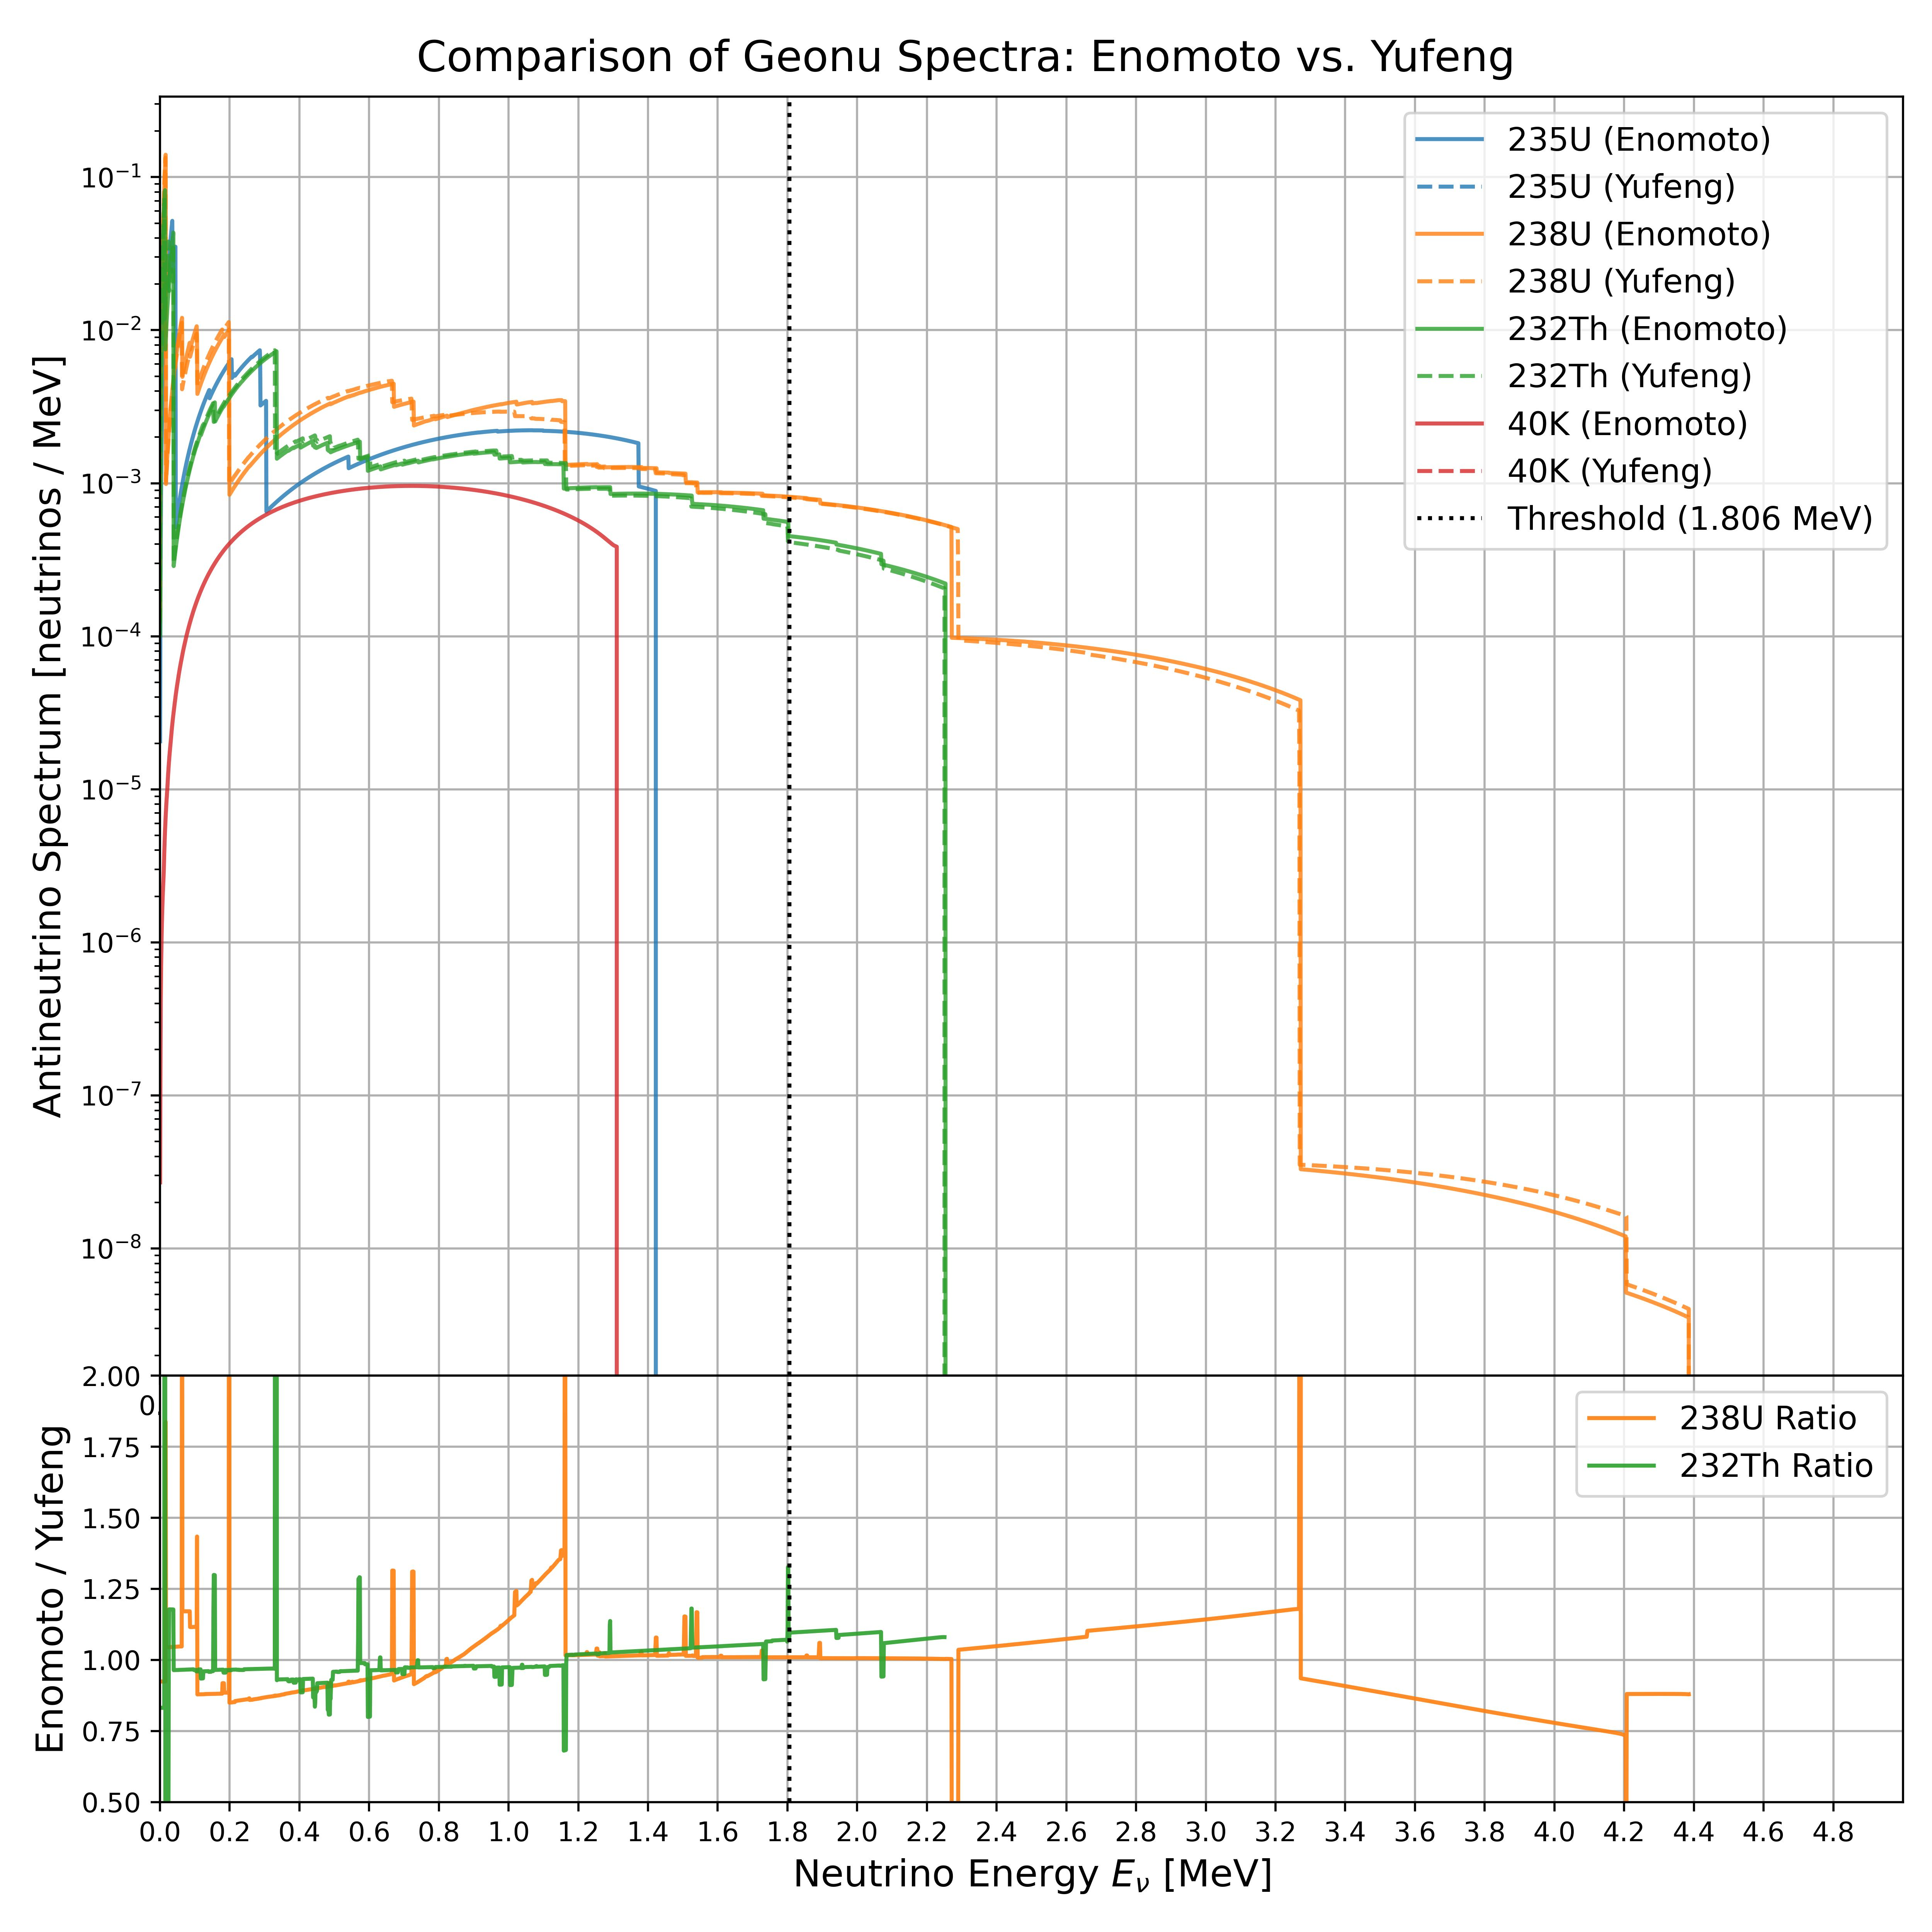
\includegraphics[scale = 0.3]{./Pics/Comparison_of_All_Geonu_Spectra.jpg}
					\caption{Spectra for different HPEs\cite{Enomoto_Spectrum,GeonSpectra-2024}}
					\label{Fig:Geonu Decay}
				\end{figure}
		\section{GEONU Software}
			GEONU is an open-source MATLAB code currently maintained by Tytrice Faison and Laura Sammon\cite{Original_GEONU}. It provides a model of the earth and is capable of computing geonu signal rates, geonu fluxex at detectors, and radiogenic power. Based on the original version, I have rewritten the entire code to improve it readability, maintainability, and modularity, making it more convenient for geonu-related researches in SNO+.\par
			GEONU models earth into three major components: Lithosphere, mantle and core. Since the core contains negligible amounts of HPEs, GEONU only considers  contributions from the lithosphere and mantle.\par
			The lithosphere is divided into sevens layers: three layers of sediment(s1, s2, s3), three layers of crust (upper crust--UC, middle crust--UC, lower crust--LC), and one layer of lithospheric mantle (LM). Each layer is discretized into $64,800$ grid cells, defined a resolution of $1^\circ \times 1^\circ$ in the longitude and latitude (see Fig. \ref{Fig:Earth Structure 1}).\par
			The mantle component contains two layers: depleted mantle (DM) and enriched mantle (EM), each also composed of $64,800$ grid cells. The averall structure of all layers is shown in Fig. \ref{Fig:Earth Structure 2}.
				\begin{figure}[H]
					\centering
					\begin{minipage}{0.49\linewidth}
						\centering
						
\includegraphics[width=0.6\linewidth]{./Pics/Earth_Structure_1.jpg}
						\caption{Layer structure division}
						\label{Fig:Earth Structure 1}
					\end{minipage}
					\begin{minipage}{0.49\linewidth}
						\center
						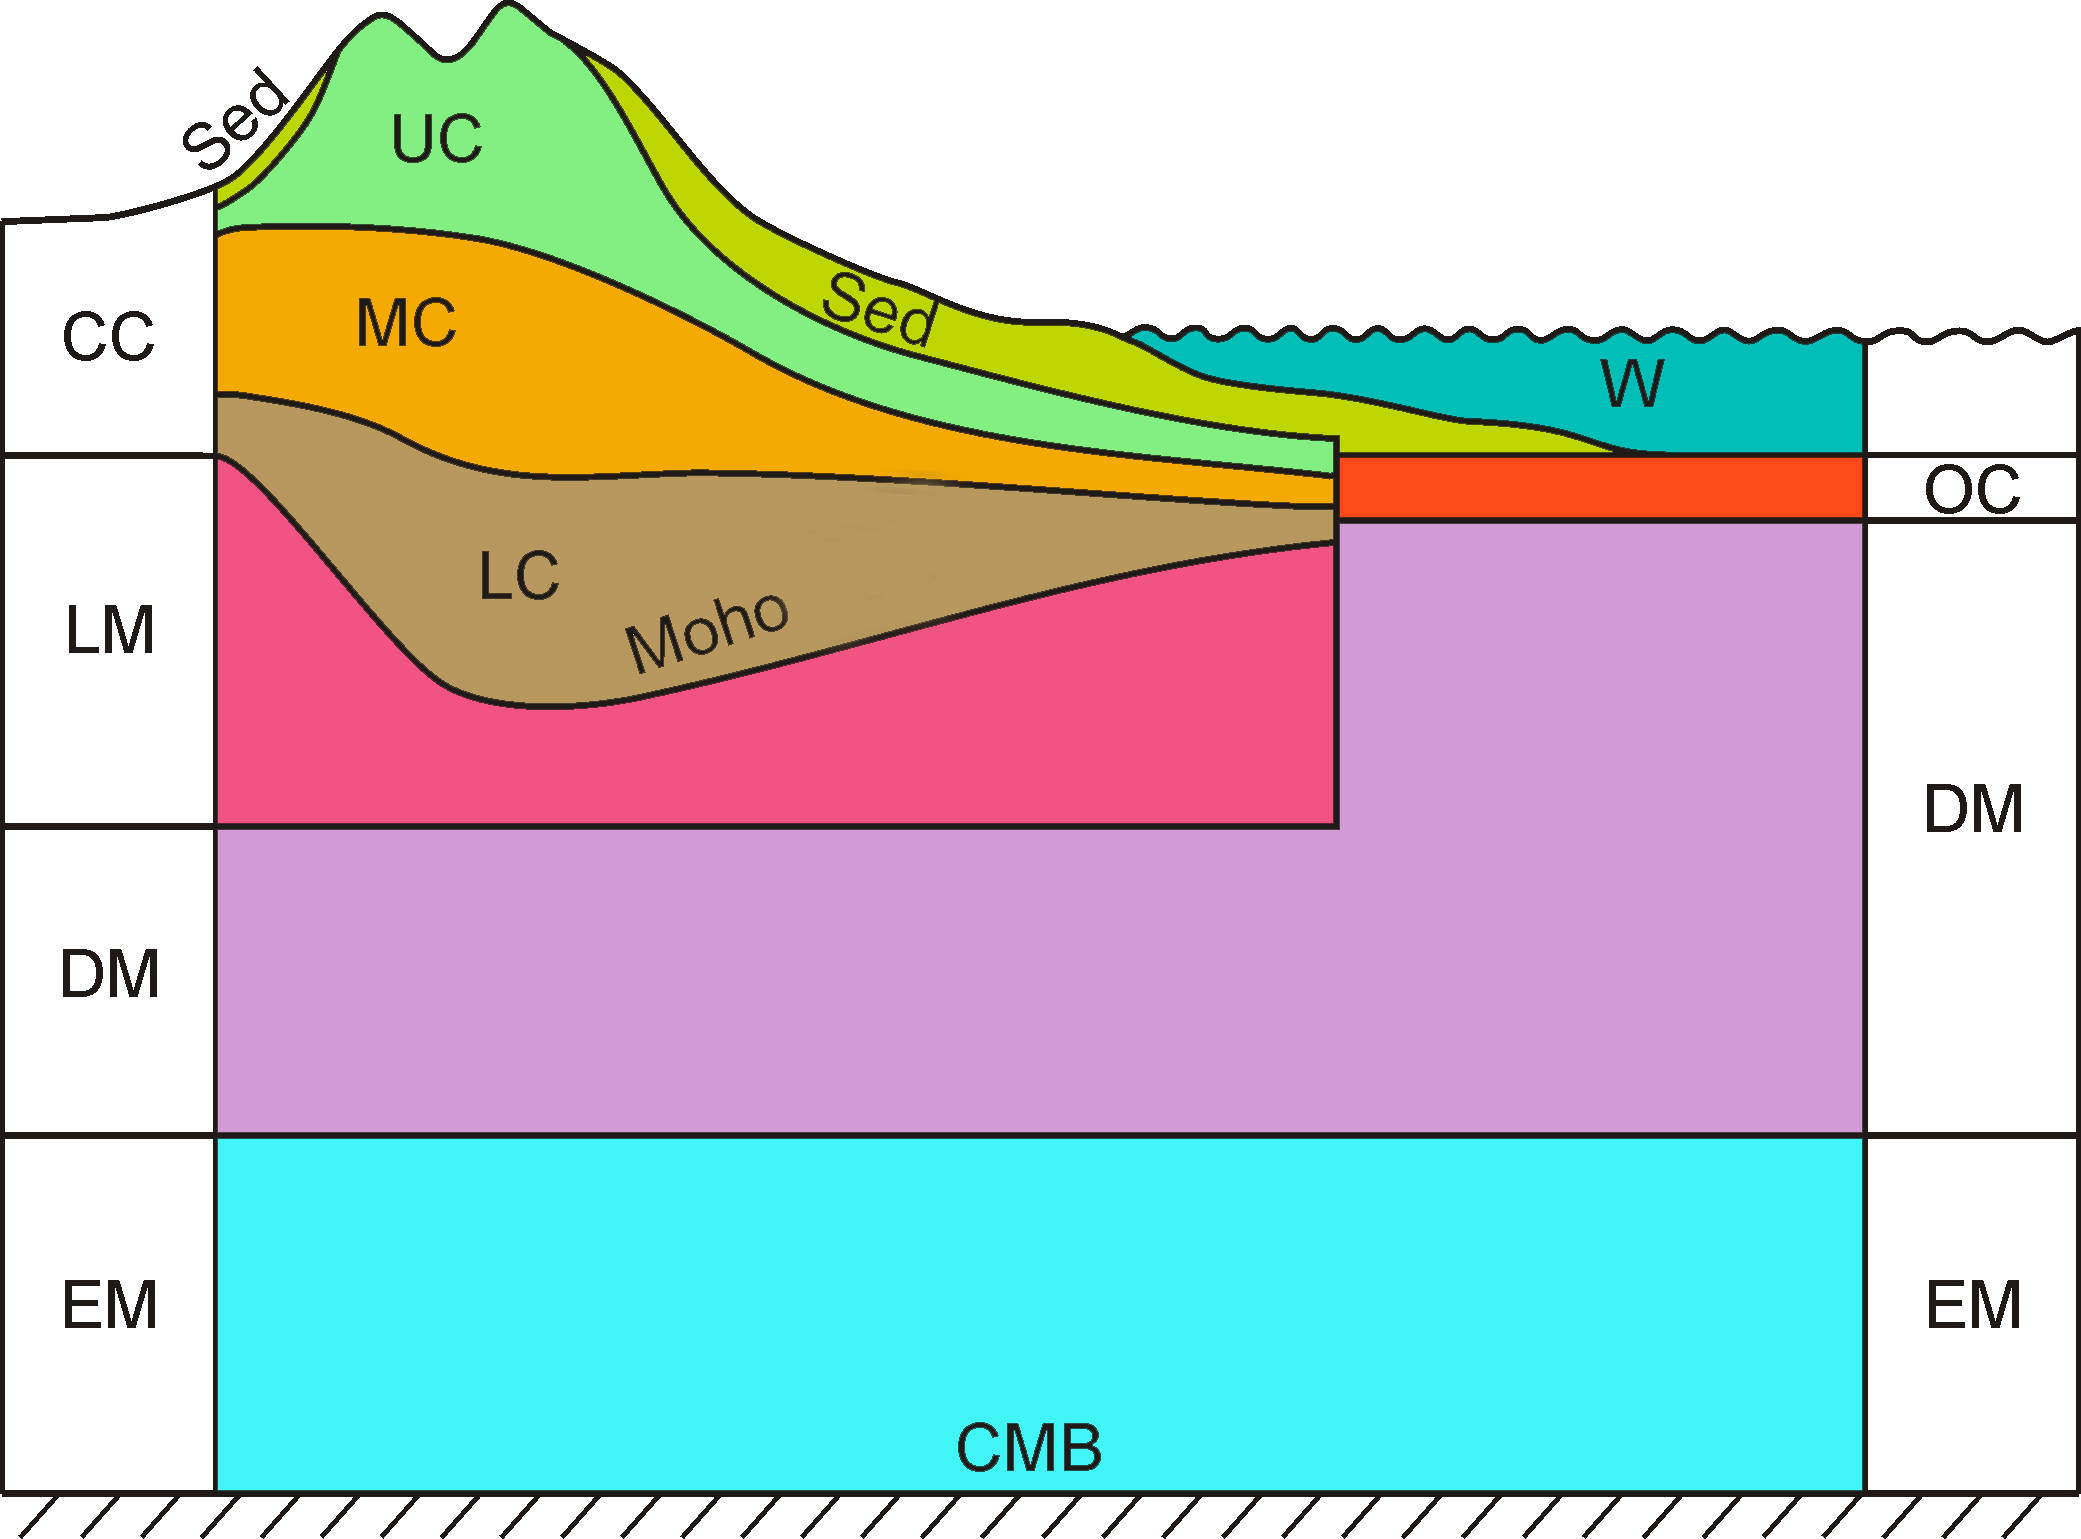
\includegraphics[width=0.8\linewidth]{./Pics/Earth_Structure_2.jpg}
						\caption{Internal structure of the Earth \cite{huang2013reference}}
						\label{Fig:Earth Structure 2}
					\end{minipage}
				\end{figure}
			In addition, GEONU requires external geological model inputs. For the lithosphere component, four models are available: Crust 1.0, Crust 2.0, Lith and ECM. For the mantle component, PREM model is used. Currently, the updated version of GEONU supports Crust 1.0 for the lithosphere and PREM for the mantle.\par
			After constructing the Earth model, the next step is to calculate the geonu signal rates. For geonu rate generated by $i$-th HPE, the calculation follows:
				\begin{equation}
					S_i
					= \int_{\oplus} \rho A_i dV \times \frac{1}{a_i} \times \frac{\ln 2}{\tau_i}\times \int \frac{dn}{dE} \sigma_{IBD} dE \times \frac{P_{ee}}{4\pi L^2} \times 1 \text{yr} \times N_{proton} \times \varepsilon_{detector},
				\end{equation}
			where $\rho$ is the rock desity; $A_i, a_i, \tau_i$ are abundance, atomic mass, and half-life of the $i$-the HPE, respectively; $P_{ee}$ is the electron antineutrino survival probability; $L$ is the distance from the source element to the detector; $N_{proton}$ is number of target protons in the detector; and $\varepsilon_{detector}$ is the detection efficiency.\par
			The geonu flux is calculated as:
				\begin{equation}
					\Phi
					= \int_{\oplus} \rho A_i dV \times \frac{1}{a_i} \times \frac{\ln 2}{\tau_i}\times \int \frac{dn}{dE} dE \times \frac{P_{ee}}{4\pi L^2},
				\end{equation}
			with units is cm$^{-2}$s$^{-1}$.\par
			The rediogenic power is derived by multiplying the total mass of each HPE with its specific power factor (i.e. heat released per unit mass). This is the framework of GEONU. More detailed methods and implementation will be introduced in the following sections.
		\section{How to use GEONU?}
			If this is your first time using GEONU software, please ensure that MATLAB is properly installed on your computer. \par
			After installation, open the \texttt{main.mlx}, select the detector of interest, set the desired number of iterations, and click the "Run" button. Since memory comsuption is strongly dependent on the number of iteration, please refer to the recommended configuration table below:
				\begin{table}[H]
					\centering
					\caption{Recommended Memory and Runtime for Different Iteration Settings}
					\begin{tabular}{|c|c|c|}
						\hline
						Iteration & Recommended Memory & Estimated Runtime\\
						\hline
						$1000$ & $32$ GB & $102$ s\\
						\hline
						$4000$ & $64$ GB & $280$ s\\
						\hline
					\end{tabular}
				\end{table}
			After the simulation finishes, results are stored in the \texttt{Output} folder. The output file contains three structures: \texttt{Physics}, \texttt{Geology}, and \texttt{Output}. The first two structures record the physics and geological input parameters, facilitating verification and reproducibility; the the \texttt{Output} stores the computed results. \par
			\texttt{Plot.m} script demostrates how to read, process and visualize the results. All generated figures are saved in the \texttt{Pics} folder.\par
			The \texttt{LITE} version demostrates the fundamental computational framework. Both \texttt{ADVANCE} and \texttt{SPECTRUM} versions are extended from it. If you plan to modify or develop your own version, \texttt{LITE} version is an excellent reference. To control the memory consumption, the following versions are released:
				\begin{itemize}
					\item \textbf{LITE:} Focuses on signal rate computation
					\item \textbf{ADVANCE:} Computes signal rate, flux, and radiogenic power.
					\item \textbf{SPECTRUM:} Compute signal rate and detected spectra.
					\item \textbf{APPLICATION:} For user-defined development and customized applications.
				\end{itemize}
			{\color{red} \textbf{INPORTANCE:} If any results from either the original or the new GEONU software are used in your publication, please cite this reference \cite{wipperfurth2020reference}, which is the first one introduced the code.}
	\chapter{Geology Information(TBA)}
		\section{Huang Method}
		\label{Geology: Huang Method}
			Huang method is based on ~\cite{Huang2013} and incorporates with the following geological observations: 1) There is an negative correlation between seismic velocities ($V_p$ and $V_s$) and SiO$_2$ content of the rocks; 2) Due to differences in temperature and pressure, the MC and LC are predominantly composed of amphibolite facies and grabulite facies, respectively. \par
			Furthermore, each rock facies can be subdivided into felsic, intermediate, and mafic types based on their SiO$_2$ content. Huang et al. assume that the amphibolite and granulite are mixtures of felsic and mafic components, with fraction $f$ and $m$, respectively. They measured the seismic velocities of these rock types and adjusted the fractions to match the observed average seismic velocities of crust. This leads to the following system of equations:
				\begin{equation}
					f + m = 1,
					\quad
					fV_{f, p} + mV_{m, p}
					= V_\mathrm{crust}.
				\end{equation}
			Finally, the abundances in MC and LC are calculated using a linear combination of the abundances in felsic and mafic rocks:
				\begin{equation}
					a = fa_f + ma_m
				\end{equation}
			where $a$ is the abundance in the crust layer, and $a_f$ and $a_m$ are the abundances in felsic and mafic rocks, respectively.\par
			It's important to note that abundances follow a log-normal distribution instead of Gaussian distribution. The GEONU adopts the following parameters:
				\begin{table}[H]
					\centering
					\caption{Iinputs in Huang Method}
					\begin{tabular}{c|c|c|c|c|c|c|c|c|c}
						\hline
						\hline
						Rock & $\mu_\mathrm{U}$(ppm) & $+\Delta_\mathrm{U}$ & $-\Delta_\mathrm{U}$ & $\mu_\mathrm{Th}$(ppm) & $+\Delta_\mathrm{Th}$ & $-\Delta_\mathrm{Th}$ & $\mu_\mathrm{K_2O}$ (wt\%)& $+\Delta_\mathrm{K_2O}$ & $-\Delta_\mathrm{K_2O}$\\
						\hline
						Amphibolite: Felsic & $1.37$ & $1.03$ & $0.59$ & $8.27$ & $8.12$ & $4.10$ & $2.89$ & $1.81$ & $1.11$\\
						\hline
						Amphibolite: Mafic & $0.37$ & $0.39$ & $0.19$ & $0.58$ & $0.57$ & $0.29$ & $0.50$ & $0.41$ & $0.23$\\
						\hline
						Granulite: Felsic & $0.42$ & $0.41$ & $0.21$ & $0.387$ & $7.35$ & $2.54$ & $2.71$ & $2.05$ & $1.17$\\
						\hline
						Granulite: Mafic & $0.10$ & $0.14$ & $0.06$ & $0.30$ & $0.46$ & $0.18$ & $0.39$ & $0.31$ & $0.17$\\
						\hline
						\hline
					\end{tabular}
				\end{table}
				\begin{figure}[H]
					\centering
					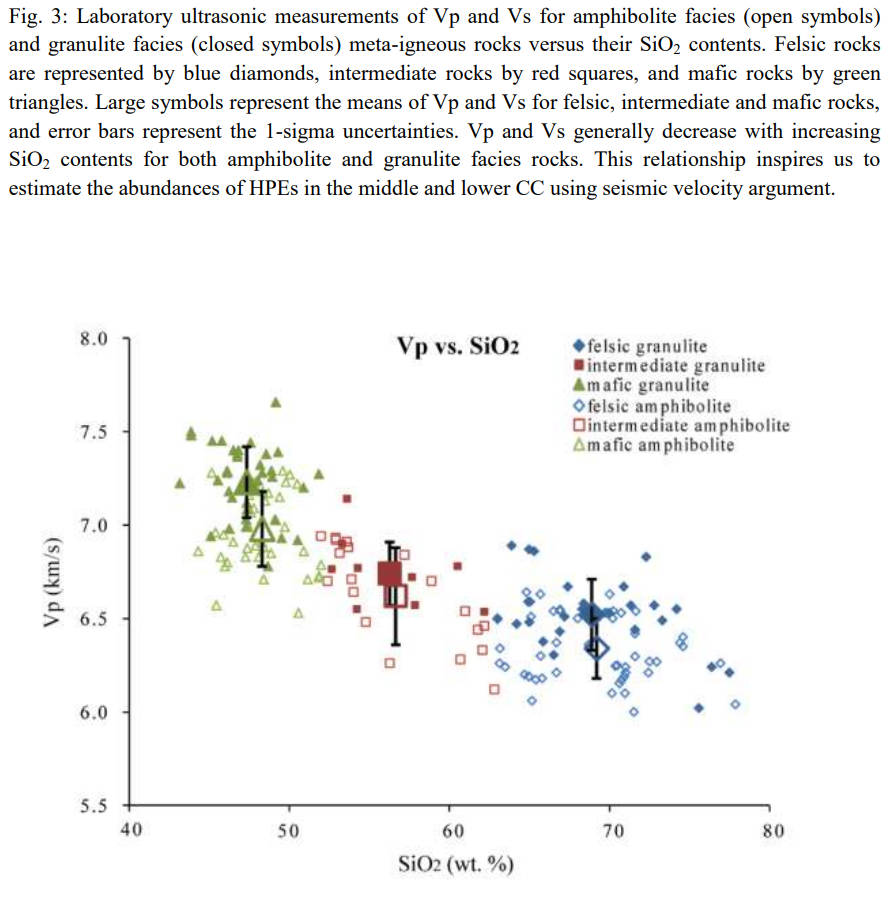
\includegraphics[scale = 0.27]{./Pics/Pic-Vp_SiO2.jpg}
					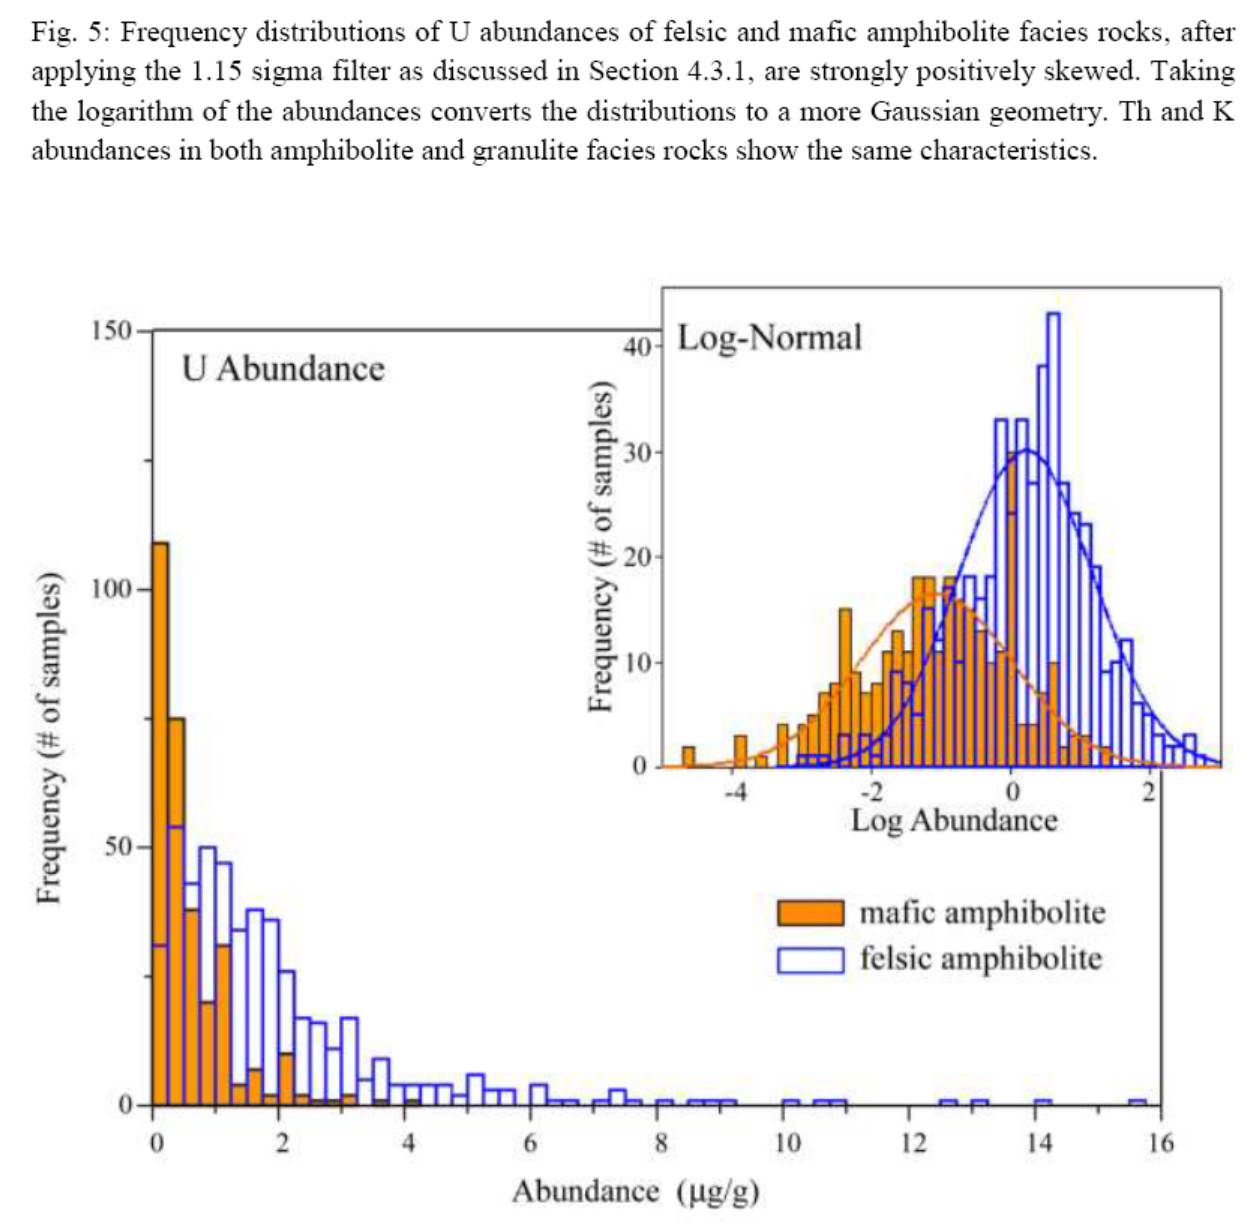
\includegraphics[scale = 0.2]{./Pics/Pic-Abundance_Distribution.jpg}
				\end{figure}
		\section{Bivart Method}
		\label{Geology: Bivart Method}
		\section{Crust 1.0}
		\section{Crust 2.0}
		\section{Litho 1}
		\section{ECM}
		
	\chapter{Input Parameters}
		\section{Physics Parameters}
			The following physical parameters are required as input:
				\begin{enumerate}
					\item \textbf{Element properties:} Detailed values are provided in Table~\ref{Table: Element Properties}.
					\item \textbf{Neutrino oscillation:} The oscillation parameters are listed in Table~\ref{Table: Oscillation Parameters}. The survival probability is given by:
					\begin{equation}
						\begin{aligned}
							P_{ee}(E, L)
							= 1  
							&- \sin^2 2\theta_{12}\cos^4 \theta_{13} \sin^2\left(\frac{1.27 \Delta m_{21}^2 L}{E}\right) \\
							&- \sin^2 2\theta_{13}\cos^2 \theta_{12} \sin^2\left(\frac{1.27 \Delta m_{31}^2 L}{E}\right) \\
							&- \sin^2 2\theta_{13}\sin^2 \theta_{12} \sin^2\left(\frac{1.27 \Delta m_{32}^2 L}{E}\right),
						\end{aligned}
					\end{equation}
					where $E$ and $L$ are neutrino energy and distance, in units of MeV and km, respectively.
					\item \textbf{Emitted neutrino spectra of HPEs:} The geoneutrino spectra currently used in most studies are calculated by Enomoto \cite{Enomoto_Spectrum}. Yufeng later provided update spectra~\cite{GeonSpectra-2024}, incorporating forbidden transitions and higher order correction. A comparison between the old and new spectra is shown in Fig.~\ref{Fig:Geonu Decay}. The updated spectra lead to reduced geonu signals, with a decrease of $3.47\%$ for uranium and $9.00\%$ for thorium.
						\begin{figure}[H]
							\centering
							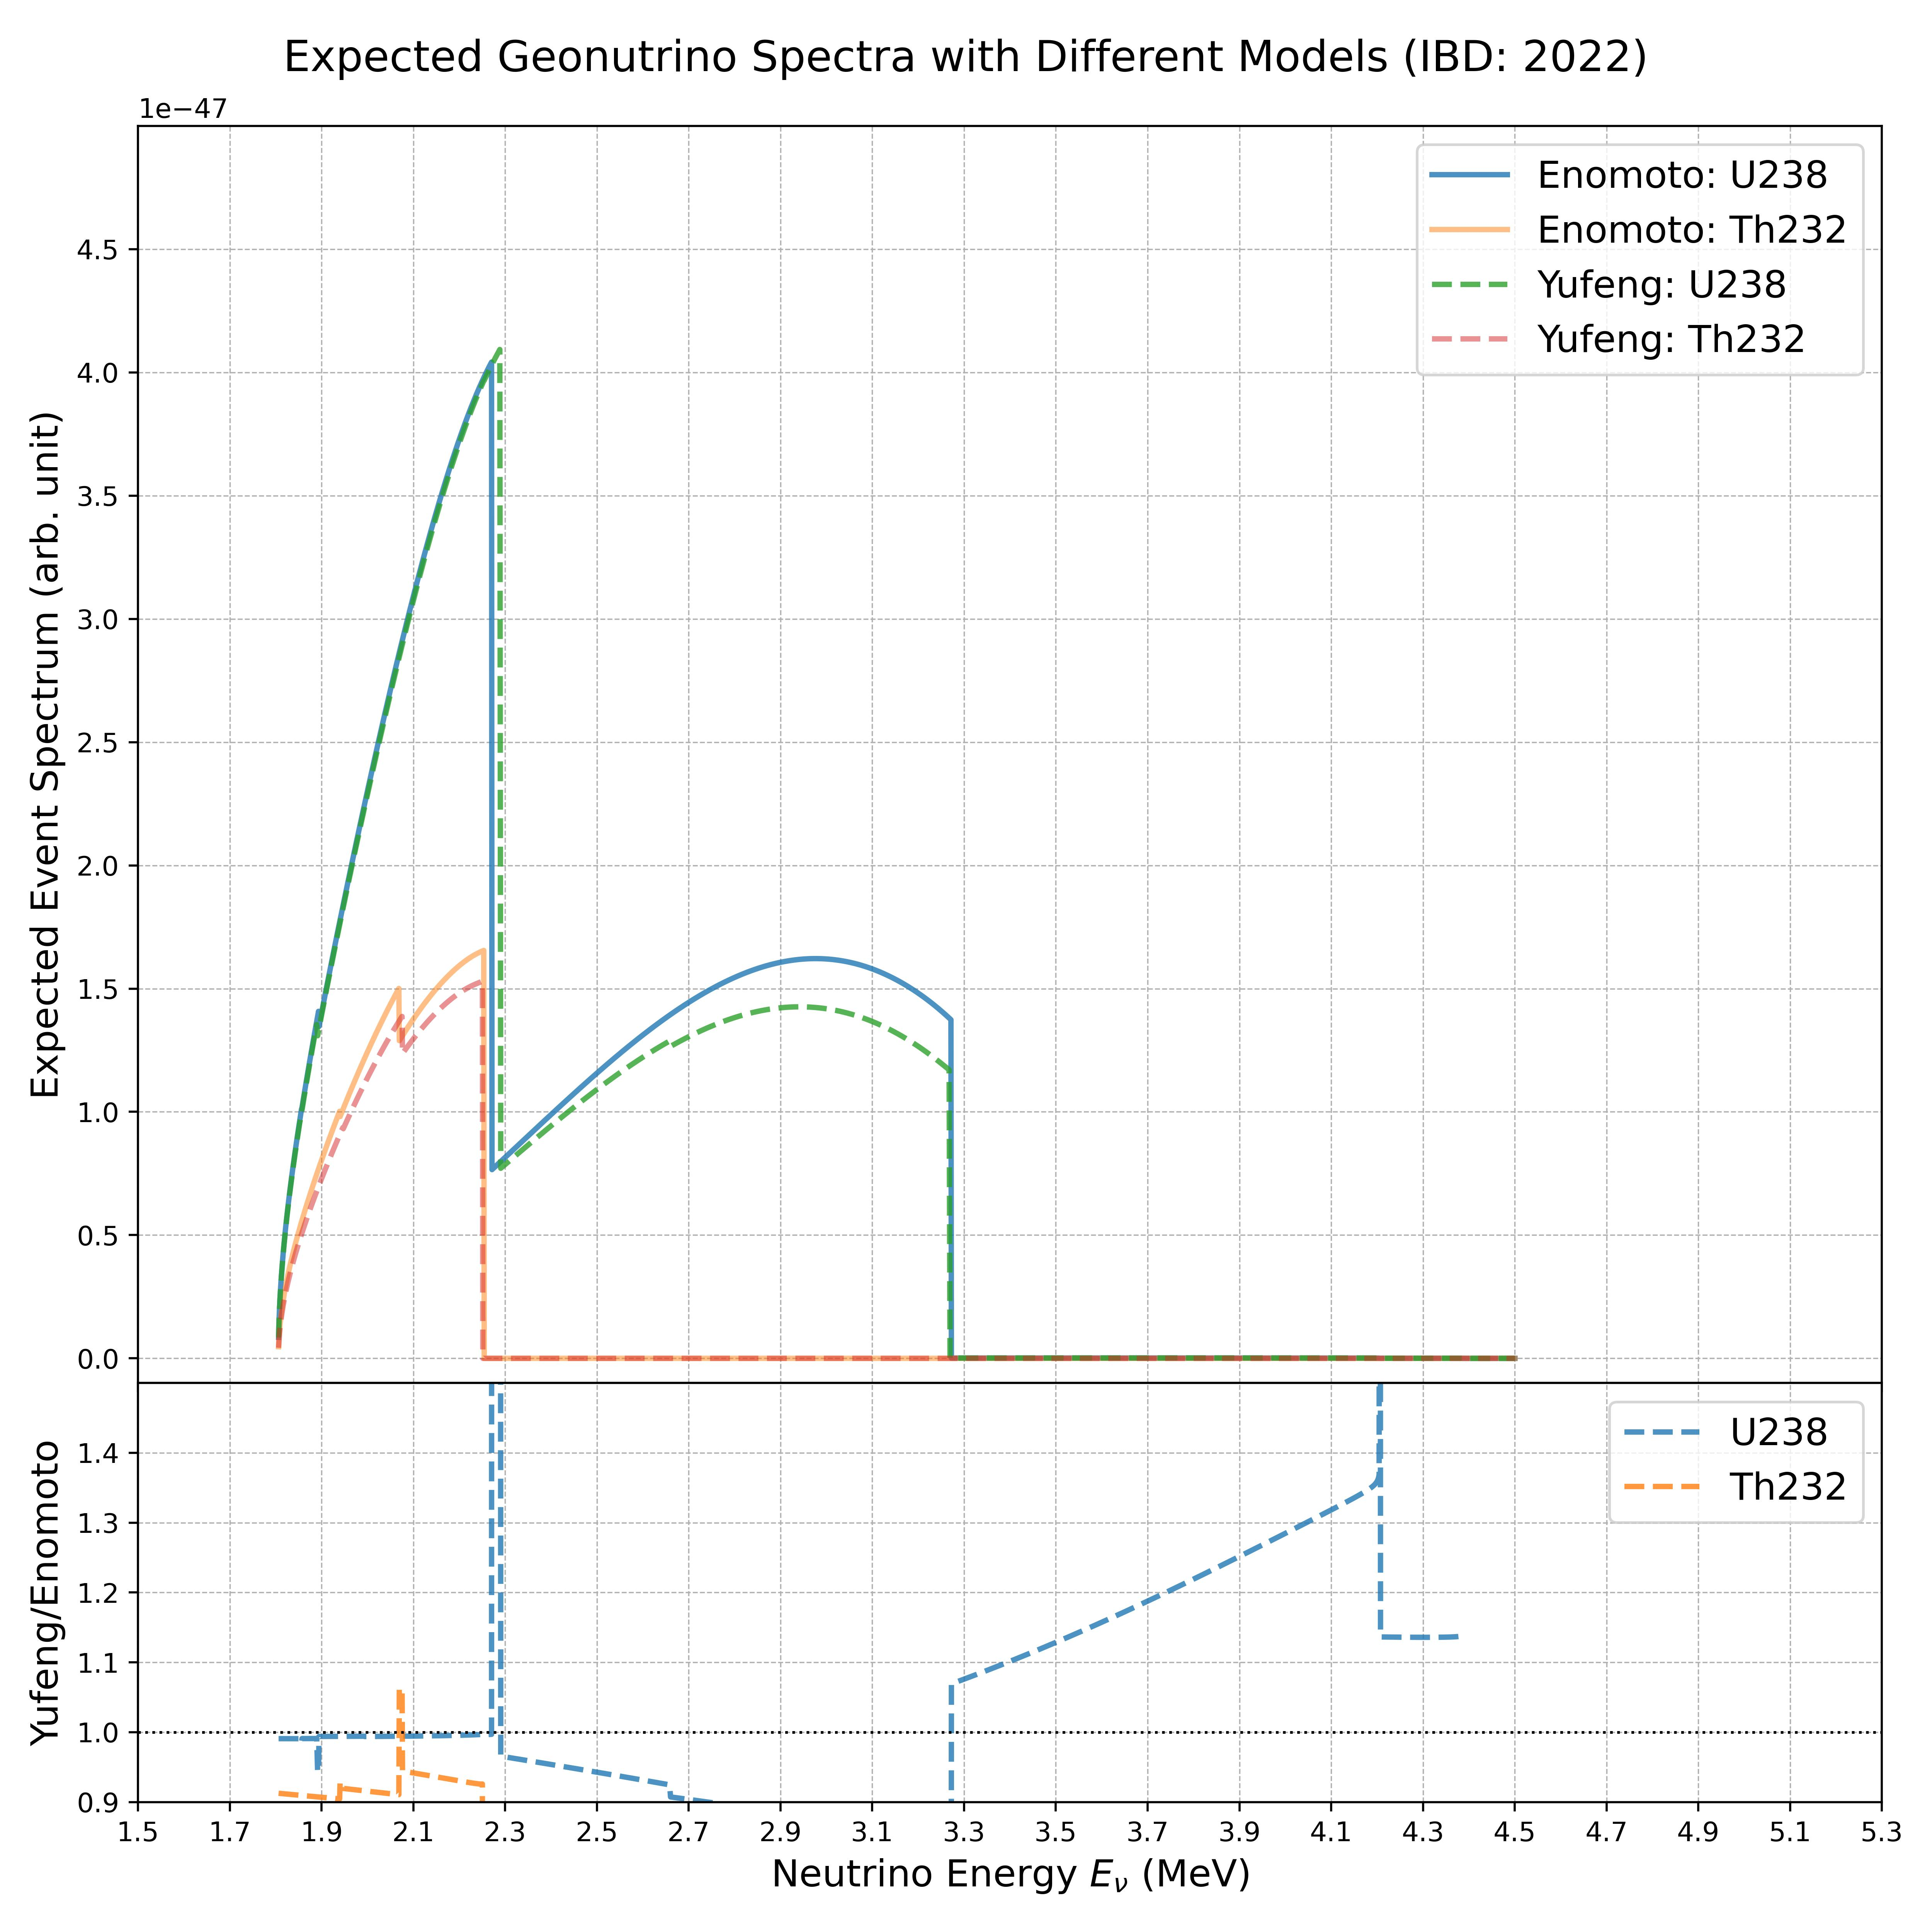
\includegraphics[scale = 0.5]{./Pics/Comparison_All_Expected_Geonu_Spectra_IBD_2022.jpg}
						\end{figure}
					\item \textbf{IBD cross-section:} GEONU supports four different formulations of the IBD cross section. All croo section data are stored in \texttt{./Input\_Files/IBD\_Cross\_Section.mat}. The four options are: \par
					1) \texttt{Approximation}: This is the most commonly used formula in geonu modeling studies, given by				
						\begin{equation}
							\sigma_{IBD}(E)
							= 9.52 \times (E - \Delta)^2 \sqrt{1 - \frac{m_e^2}{(E - \Delta)^2}} \times 10^{-44} \text{cm}^2,
						\end{equation}
					where $\Delta \equiv m_n - m_p \approx 1.2933$ MeV.\par
					2) \texttt{Vogel \& Beacom (1999)}: This calculation is based on~\cite{IBD-1999}. The paper includes effects of nucleon recoil and weak magnetism, and derive a first-order asymptotic expression via Taylor expansion in the limit $M\rightarrow \infty$.\par
					3) \texttt{Strumia \& Vissani (2003)}: This is based on~\cite{IBD-2003}. The authors perform a full relativistic calculation, incorporating four form factors: $f_1, f_2, g_1$ and $g_2$. The uncertainty in the low-energy region is estimated to be approximately $0.4\%$.\par
					4) \texttt{Vissani et al. (2022)}: This calculation is based on ~\cite{IBD-2022}. The study includes the second-class current associated with $f_3$ and $g_3$ based on~\cite{IBD-2003}, and estimates the uncertainty in the low-energy region to be about $0.094\%$.
						\begin{figure}[H]
							\centering
							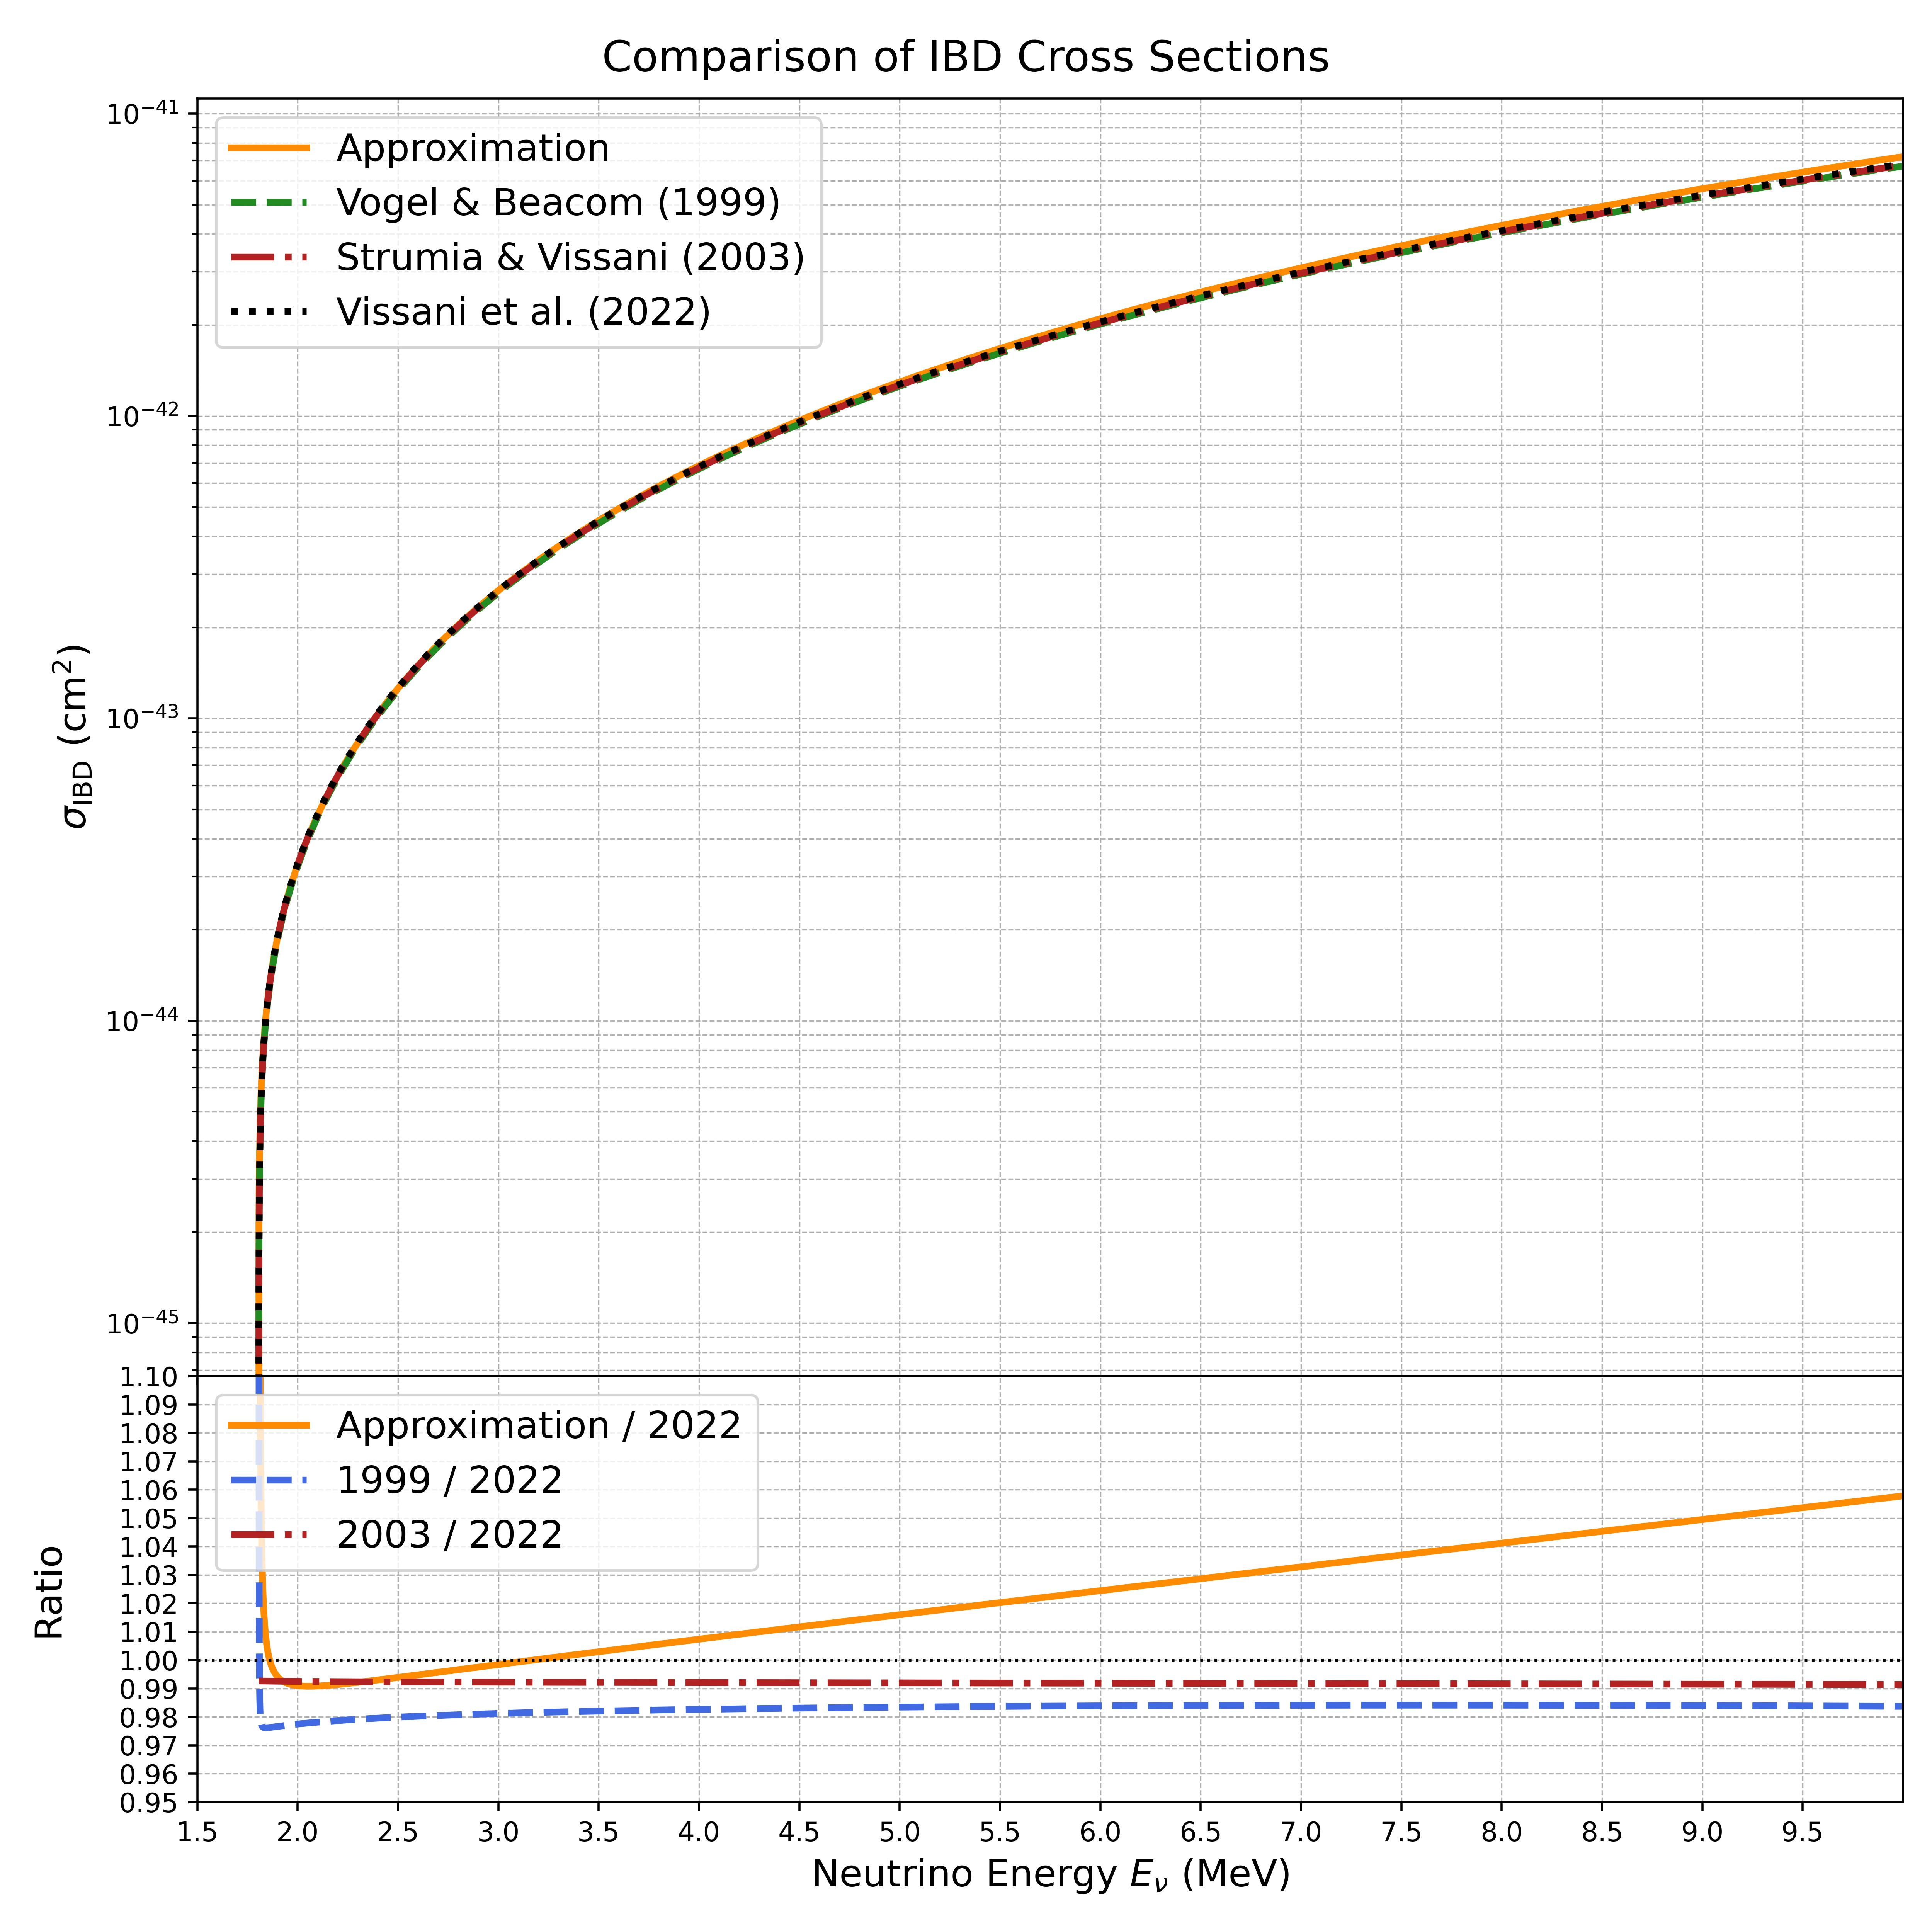
\includegraphics[scale = 0.5]{./Pics/Comparison_of_All_Computed_IBD_Cross_Section.jpg}
						\end{figure}
				\end{enumerate}
				\begin{table}[H]
					\centering
					\caption{Element Properties}
					\begin{tabular}{p{3.5cm}|p{2cm}p{2cm}p{2cm}p{3cm}|p{2cm}}
						\hline
						\hline
						Property & ${}^{235}$U & ${}^{238}$U & ${}^{232}$Th & ${}^{40}$K & Reference\\
						\hline
						Natural abundance & $0.7\%$ & $99.3\%$ & $100\%$ & $0.0117\%$ & Wiki\\
						\hline
						Atomic mass (amu) & $235.0439299$& $238.05078826$ & $232.0380536$ & $39.96399848165$ & Wiki \\
						\hline
						Half-life (s)/$3.1536$e$7$ & $4.468$e$9$ & $0.704$e$9$ & $14.05$e$9$ & $1.248$e$9$ & Wiki \\
						\hline
						Heat power ($\mu$W/kg) & $568.48$ & $95.13$ & $26.28$ & $24.47$ & Ref \cite{dye2012geoneutrinos}\\
						\hline
						\hline
					\end{tabular}
					\label{Table: Element Properties}
				\end{table}
				\begin{table}[H]
					\centering
					\caption{Neutrino Oscillation Parameters (PDG 2024)}
					\begin{tabular}{p{2.5cm}|p{3cm}|p{5cm}|p{3cm}}
						\hline
						\hline
						Mixing Angle & Value & Mass-Square Difference($\text{eV}^2$) & Value\\
						\hline
						$\sin^2 \theta_{13}/10^{-2}$ & $2.203\pm 0.059$ & $\Delta m_{21}^2/10^{-5}$ & $7.41\pm 0.21$\\
						\hline
						$\sin^2 \theta_{12}/10^{-1}$ & $3.03\pm 0.12$ & $\Delta m_{31}^2/10^{-3}$ & $2.437\pm 0.028$\\
						\hline
						$\sin^2 \theta_{23}/10^{-1}$ & $5.72\pm 0.23$ & $\Delta m_{32}^2/10^{-3}$ & $2.437\pm 0.028$\\
						\hline
						\hline
					\end{tabular}
					\label{Table: Oscillation Parameters}
				\end{table}
				\begin{table}[H]
					\centering
					\caption{Electron and Nucleon Masses}
					\begin{tabular}{p{3cm}p{3cm}p{3cm}|p{3cm}}
						\hline
						\hline
						$m_e$(MeV) & $m_p$(MeV) & $m_n$(MeV) & Reference\\
						\hline
						$0.51099895069$ & $938.27208943$ & $939.56542052$ & Wiki\\
						\hline
						\hline
					\end{tabular}
					\label{Table: Electron and Nucleon Mass}
				\end{table}
		\section{Geology Parameters}
			The following geological parameters are required as input:
				\begin{enumerate}
					\item \textbf{Lithospheric geological models:} GEONU currently supports Crust 1.0 model and will support Crust 2.0, Litho 1.0 and ECM1 in the future. These models provides information such as rock density, depth, thickness and other information of each grid cell.
					\item \textbf{HPE abundances in the lithospphere:} Users are required to input the mean and standard deviation of Uranium, Thorium and Potassium abundances. GEONU then samples and assigns values to each cell accordingly. For the CC portion in the MC or LC, abundances are calculated using either the Huang or Bivart method.
					\item \textbf{Mantle geological model:} GEONU incorporates the PREM model, which provides the Earth's density profile as a function of depth.
					\item \textbf{Mantle abundances:} Required inputs include U abundance and Th/U and K/U ratios for both the DM and BSE.
					\item \textbf{Other geological parameters:} Additional parameters relevant to geophysical calculations may also be specified.
				\end{enumerate}
				\begin{table}[H]
					\centering
					\caption{Default HPE Abundances in Lithosphere Layers}
					\renewcommand{\arraystretch}{1.2} % 增加表格行距
					\begin{tabular}{p{1.5cm}|p{2cm}p{2cm}p{3cm}|p{2cm}p{2cm}p{3cm}}
						\hline
						\hline
						\multirow{2}{*}{Layer} & \multicolumn{3}{c|}{CC} & \multicolumn{3}{c}{OC} \\  
						\cline{2-7}
						& U/$10^{-6}$ & Th/$10^{-6}$ & K/$10^{-2}$ & U/$10^{-6}$ & Th/$10^{-6}$ & K/$10^{-2}$\\
						\hline
						Sediment & $1.73\pm 0.09$ & $8.10\pm 0.59$ & $(2.21 \pm 0.14)* 0.83$ & $1.73 \pm 0.09$ & $8.10 \pm 0.59$ & $(2.21 \pm 0.14) * 0.83$\\
						\hline
						UC & $2.7 \pm 0.6$ & $10.5 \pm 1.0$ & $2.32 \pm 0.19$ & $0.07\pm 0.021$ & $0.21 \pm 0.063$ & $0.0716 \pm 0.0215$\\
						\hline
						MC/LC & \multicolumn{3}{c|}{Huang/Bivart} & $0.07 \pm 0.021$ & $0.21 \pm 0.063$ & $0.0716 \pm 0.0215$ \\
						\hline
						LM & $0.033^{+0.049}_{-0.020}$ & $0.15^{+0.277}_{-0.097}$ & $0.0315^{+0.04316}_{-0.01826}$ & \multicolumn{3}{c}{$0$} \\
						\hline
						\hline
					\end{tabular}
					\label{Table: Lithosphere Default Abundance Input}
				\end{table}
				\begin{table}[H]
					\centering
					\caption{Default HPE Abundances in BSE}
					\begin{tabular}{p{3cm}p{3cm}p{3cm}}
						\hline
						\hline
						U/$10^{-9}$ & Th/U & K/U\\
						\hline
						$19 \pm 3.8$ & $3.776^{+0.122}_{-0.075}$ & $13800 \pm 1300$\\
						\hline
						\hline
					\end{tabular}
					\label{Table: BSE Default Abundance Input}
				\end{table}
				\begin{table}[H]
					\centering
					\caption{Default Mantle Input Parameters}
					\begin{tabular}{p{3.5cm}p{3cm}p{3cm}}
						\hline
						\hline
						EM (mass fraction) & Th/U & K/U \\
						\hline
						$19\%$ & $3.45^{+1.66}_{-1.18}$ & $19000 \pm 1300$\\
						\hline
						\hline
					\end{tabular}
				\end{table}
				\begin{table}[H]
					\centering
					\caption{Other Default Geological Inputs}
					\begin{tabular}{p{4cm}|p{4cm}}
						\hline
						\hline
						Earth mass (kg)/$10^{24}$ & Core mass (kg)/$10^{24}$\\
						\hline
						$5.97218 \pm 0.00006 $ & $ 1.93265 \pm 0.0579795$\\
						\hline
						\hline
					\end{tabular}
					\label{Table: Other Default Geology Input}
				\end{table}
		\section{Parameters for Low-, Mid-, and High-Q Models (TBA)}
	\chapter{Design of Software}
		\section{Design Philosophy}
			\subsection{Monte Carlo Sampling Framework}
				One of the core design principles of GEONU is the use of Monte Carlo sampling to incorporate uncertainties in geological parameters. This is achieved through the following functions:
					\begin{enumerate}
						\item \texttt{Generate\_Random\_Normal():} Performs Gaussian sampling based on mean and standard deviation.
						\item \texttt{Generate\_Random\_Log\_Normal():} Performs log-normal sampling.
					\end{enumerate}
				These sampling methods allow GEONU to account for input uncertainties and propagate them through the entire calculation. In addition, GEONU uses correlation coefficients in sampling to make a more realistic simulation.
			\subsection{Statistics and Error}
				In the original GEONU software, the function \texttt{Abund\_And\_Flux()} invoked \texttt{stat()} and similar functions to perform statistical analysis immediately after computation. However, this approach significantly slowed down the programm and  randomness of the overall results. In the updated version of GEONU, all statistical operations have been completely removed from the computation phase. Statistical analysis is now applied only to the final results in subsequent post-processing steps. For pratical implementation, refer to \texttt{./Plot.m}.
		\section{Physics}
			All functions related to physics are stored in \texttt{./Functions/Physics}, and are summarized as follows:
				\begin{enumerate}
					\item \texttt{Compute\_Relative\_Abundance\_Mass():} This function computes the natural abundance by mass of the element. For example, in GEONU, the input and computed abundance of uranium refers to the total abundance, whereas uranium consist of ${}^{238}$U and ${}^{235}$U. This funciton calculates the contribution of ${}^{238}$U from the total abundance.
					\item \texttt{Load\_Oscillation\_Parameters():} This function stores the default oscillation parameters. It also includes a flag \texttt{Physics.Oscillation.Constant} to control whether random sampling of the oscillation parameters is applied; however, this feature is currently distabled. At end of the function, three variables \texttt{p1, p2, p3} are computed as:
						\begin{align}
							p1 = -\sin^2 2\theta_{12} \cos^4 \theta_{13},
							\quad
							p2 = -\sin^2 2\theta_{13} \cos^2 \theta_{12},
							\quad
							p3 = - \sin^2 2\theta_{13} \sin^2 \theta_{12}.
						\end{align}
					These variables simplify the neutrino oscillation calculation and improve the code's readability and maintainability.
					\item \texttt{Load\_Geonu\_Spectrum():} This function loads the neutrino spectra from decay of HPEs. The original spectra have units of keV and 1/keV. To boost  simulation and consider the limit to the energy resolution of the detector, the spectra re resummed. Currently, only the energy range from $0-3.5$ MeV with a bin width of $0.1$ MeV is considered.
					\item \texttt{Compute\_Cross\_Section():} This function loads IBD cross-section.
					\item \texttt{Compute\_Signal\_Response():} This function computes the signal rate response, $g_i$, for ${}^{238}$U and ${}^{232}$Th, defined as:
						\begin{equation}
							g_i
							\equiv \frac{1}{4\pi}\frac{1}{a_i} \frac{\ln(2)}{\tau_i} \left(\frac{dn}{dE}\right) \sigma_{IBD} \times 1 \textbf{yr} \times 10^{32} \times \frac{1}{10^4},
						\end{equation}
					where the factor $10^{-4}$ accounts for the unit conversion form $cm^2$ to $m^2$. Consequently, the geonu signal rate is computed as:
						\begin{equation}
							S
							= \int_{\oplus} \rho A_i dV \times g_i \times \frac{P_{ee}}{L^2}.
						\end{equation}
					\item \texttt{Load\_Detector():} This function loads information of the detectors, including 1) longitude; 2) latitude; 3) depth (m); 4) detection efficiency; 5) target proton number; 6) longitude and latitude of the grid cell closet to the detector; 7) detector name.
				\end{enumerate}
		\section{Lithosphere}
			All scripts and functions related to the Lithosphere are stored in \texttt{./Functions/Geology}, \\ \texttt{./Functions/Computation/Lithosphere}, and \texttt{./Functions/Computation/DeepCrust}. The first directory involves geological inputs before computation, while the last two refer to the computational details.\par
			The script\texttt{./Functions/Geology/Setting\_Asign.m} records the abundance inputs for each lithospheric layer and call almost all functions under \texttt{./Functions/Geology}. Their names and purposes are summarized as follow:
				\begin{enumerate}
					\item \texttt{Load\_Lithosphere\_Data():} This function first loads specified geological model. Then it calls \texttt{Assign\_OC\_CC()} to classify the grid cells according to the model, indentifying which cells belong to the CC and which to the OC. This classification directly affects how abundances are assigned and how signals are calculated in later steps. Finally, it calls \texttt{Preallocate\_Variables\_Lithosphere()} to define the data structure for PHEs in each layer: each row represents a grid cell with three columns--(1) mean value, (2) positive error, and (3) negative error.
					\item \texttt{Generate\_Correlations():} This function generates the correlation efficients used for sampling. For Bivart method, the correlation coefficients involving SiO$_2$ are handled separately in \\ \texttt{Generate\_Correlations\_DeepCrust()}.
					\item \texttt{Compute\_Abundance\_DeepCrust():} This function produces the data needed for the Huang method and loads datasets required for the Bivart method. It is important to note that, in the Huang method, the potassium abundance is given as the weight fraction (wt\%) of K${}_2$O instead of in g/g units. Therefore, a conversion using \texttt{wt} and \texttt{K2O} is needed to obtain the final potassium abundance.
					\item \texttt{Assign\_Abundance\_Layer():} This function assigns HPE abundances to all grid cells.
					\item \texttt{Compute\_Abundance\_BSE():} This function computes HPE abundances for the BSE model.
					\item \texttt{Find\_Near\_Cells():} This function was originally designed to find the grid cells nearest to the detector. However, it is currently disabled and will not be used in the future.
				\end{enumerate}
			\par
			The script \texttt{./Functions/Computation/Lithosphere/Generate\_Temp\_Variables\_For\_Parallel.m} defines the variables required during the computation process, including the initialization of \texttt{array\_for\_signal}.\par
			The script \texttt{./Functions/Computation/Lithosphere/Compute\_Temp\_Variables.m} computes template variables for different layers.\par
			The script \texttt{./Functions/Output/LITE/Record\_Lithosphere\_Results.m} records output data, which can be customized for specific needs.\par
			The script \texttt{LITE\_Compute\_Lithosphere\_Cell()} serves as the core function of GEONU, responsible for (1) computing abundance, (2) subdividing grid cells, and (3) calculating signal rates. The input variables are outlined as follow:
				\begin{enumerate}
					\item \texttt{index:} Index of the grid cell, primarily used for debugging purposes.
					\item \texttt{Iteration:} Number of iterations, used to define the size of matrices.
					\item \texttt{name\_model:} The name of method applied for Deepcrust calculations.
					\item \texttt{name\_layer:} The name of layer; certain layers require special handing.
					\item \texttt{last\_layer\_pressure:} Pressure from last layer, necessary for Huang method.
					\item \texttt{cor\_array:} Correlation efficients required in Monte Carlo sampling.
					\item \texttt{array\_for\_radius,array\_for\_mass,array\_for\_abundance,array\_for\_signal:} Structures containing information related to radius, mass, abundance, and signal rate computations, respectively.
					\item \texttt{detector:} Detector information.
				\end{enumerate}
			The output variables are outlined as follows:
				\begin{enumerate}
					\item \texttt{TOTAL\_MASS, MASS\_U, MASS\_TH:} Mass of the rock (kg), uranium (kg), and thorium (kg), respectively. These quantities are used to calculate the masses in the mantle.
					\item \texttt{PRESSURE\_TO\_LAYER:} The pressure value required for pressure correction in the Huang method. This value will be passed to the next layer during abundance calculations.
				\end{enumerate}
			A general computational framework is adopted, which helps to understand the main logic as there are various cases handled in this function. This framework applies to s1-s3, UC, MC\_CC, LC\_CC, and LM\_CC layers; other layers require special treatments, which will be described separately. The general framework is outlined as follow:
				\begin{enumerate}
					\item \textbf{Thickness check:} If the thickness of the layer is $0$, the computation terminates immediately and returns zero values for outputs.
					\item \texttt{MASS\_TOTAL:} The radius of the grid cell is calculated based on the rock depth and thickness. The rock density is then sampled according to the specified statistical model, and the total rock mass of the grid cell is computed.
					\item \texttt{PRESSURE:} The pressure increment from this grid cell is computed as $\Delta p_i = \rho_i g h_i$. The total pressure at the center of the grid cell is given by $p_{i - 1} + \Delta p_i/2$, and the pressure propagated to the next grid cell is $p_i = p_{i - 1} + \Delta p_i$.
					\item \texttt{ABUNDANCE:} The abundances of HPEs are sampled using either Gaussian or log-normal distributions, depending on \texttt{array\_for\_abuance}.
					\item \texttt{MASS\_U, MASS\_TH:} The total masses of the uranium and thorium are computed as $m_i = A_i \times M$.
					\item \texttt{SIGNAL\_U, SIGNAL\_TH:} GEONU first computes the distance from the grid cell to the detector. Based on the distance, the grid cell may be subdivided up to two times to improve accuracy. Each subdivided volume element $j$ contributes to the \texttt{geonu\_factor} $G_i$ defined as:
						\begin{equation}
							G_i
							\equiv \sum_j \Delta V_j \times g_j \times \frac{P_{j, ee}}{L_j^2},
						\end{equation}
					where $j$ is the index of subdivided cell. Finally the signal from this grid cell is given by:
						\begin{equation}
							\Delta S_i
							= \rho_i A_i \Delta V_i \times g_i \times \frac{P_{ee}}{L^2}
							= \rho_i A_i G_i.
						\end{equation}
				\end{enumerate}
			This marks the end of the general framework. Special cases are handled as follow:
				\begin{enumerate}
					\item \texttt{LM\_OC:} The function immediately terminates and returns zero values for this layer, as such a geological structure doesn't exist in reality.
					\item \texttt{LM\_CC} in Crust1.0 and Crust2.0: The thickness of this layer is calculated using the LAB and Moho boundaries. The underlying reason for this treatment remains unclear at present and requires further investigation.
					\item \texttt{MC\_CC} and \texttt{LC\_CC}: The abundances in these layers are computed by Huang or Bivart method, which are described in Sections~\ref{Geology: Huang Method} and Sections~\ref{Geology: Bivart Method}, respectively. The variables \texttt{PRESSURE} and \texttt{TEMPERATURE} are used in the Huang method.
				\end{enumerate}
			Finally, the manuscript \texttt{./Fuctions/Computation/Lithsophere/LITE/Clear\_Template\_Variables.m} is designed to clear intermediate variables and release memory.
				\begin{table}[H]
					\centering
					\caption{Inputs for Different Layers: \texttt{array\_for\_radius, array\_for\_mass}}
					\begin{tabular}{p{3cm}|p{2cm}p{2cm}p{2cm}p{3cm}}
						\hline
						\hline
						Layers & 1 & 2 & 3 & 4\\
						\hline
						Sed, Crust & \texttt{thick} & $0$ & \texttt{depth} & \texttt{surface\_radius}\\
						\hline
						LM & \texttt{thick} & \texttt{moho} & \texttt{depth} & \texttt{surface\_radius}\\
						\hline
						\hline
					\end{tabular}
				\end{table}
				\begin{table}[H]
					\centering
					\caption{Inputs for Different Layers: \texttt{cor\_array}}
					\begin{tabular}{p{6cm}|p{2cm}p{2cm}p{2cm}p{2cm}}
						\hline
						\hline
						Layer & 1 & 2 & 3 & 4\\
						\hline
						Sed, UC, MC\_OC, LC\_OC, LM & thick & vp & abund & -\\
						\hline
						Huang: MC\_CC, LC\_CC & thick & vp & end & -\\
						\hline
						Bivart: MC\_CC, LC\_CC & thick & vp & biv\_sio2 & biv\_abund\\
						\hline
						\hline
					\end{tabular}
				\end{table}
				\begin{table}[H]
					\centering
					\caption{Inputs for Different Layers: \texttt{array\_for\_abund}}
					\begin{tabular}{p{3.5cm}| p{1.5cm} p{1cm} p{1.5cm} p{1cm} p{1cm} p{1.2cm} p{1cm} p{1cm} p{1cm}}
						\hline
						\hline
						Layer & 1 & 2 & 3 & 4 & 5 & 6 & 7 & 8 & 9\\
						\hline
						Sed, UC, MC\_OC, LC\_OC, LM & $a_U$ & +$\Delta a_U$ & -$\Delta a_U$ & $a_{Th}$ & +$\Delta a_{Th} $ & -$\Delta a_{Th}$ & $a_K$ & +$\Delta a_K$ & -$\Delta a_K$\\
						\hline
						Huang: MC\_CC, LC\_CC & \texttt{crust\_vp} & \texttt{method} & \texttt{f\_U} & \texttt{f\_Th} & \texttt{f\_K} & \texttt{m\_U} & \texttt{m\_Th} & \texttt{m\_K} & \texttt{K\_Ratio}\\
						\hline
						Bivart: MC\_CC & \texttt{crust\_vp} & \texttt{method} & \texttt{center\_vp} & \texttt{am\_u} & \texttt{am\_th} & \texttt{am\_k20} & \texttt{k\_k20} & - & -\\
						Bivart: LC\_CC & \texttt{crust\_vp} & \texttt{method} & \texttt{center\_vp} & \texttt{gr\_u} & \texttt{gr\_u} & \texttt{gr\_k20} & \texttt{k\_k20} & - & -\\
						\hline
						\hline
					\end{tabular}
				\end{table}
		\section{Mantle}
			Due to the lack of direct measurement, All current information about the mantle is inferred. The corresponding computation is implemented in \texttt{./Functions/Computation/Mantle/Compute\_Mantle\_Variables.m}. In GEONU, the following quantities are used:
				\begin{enumerate}
					\item \textbf{Lithosphere:} Total masses of the rock, uranium and thorium.
					\item \textbf{Earth and Core:} Sampled total masses of the Earth and its core.
					\item \textbf{BSE:} Total mass of the rock and the abundances of uranium and thorium in the BSE.
				\end{enumerate}
			Based on those inputs, the total masses of the rock, uranium and thorium can be estimated. Seismic studies suggest that the mantle consists of two components: depleted mantle (DM) and enriched mantle (EM), with a commonly assumed mass ratio of $81:19$. This ratio can be adjusted via the parameter \texttt{Geology.Mantle.Proption\_EM}.\par
			A reference uranium abundance of $a_U = 8 \pm 2.4$ is adopted for DM, and two scenarios are considered accordingly:
				\begin{enumerate}
					\item \textbf{Ideal case:} If the total uranium mass in the mantle exceeds the amount required by DM at this reference abundance, GEONU assigns $a_U$ to DM.
					\item \textbf{Non-ideal case:} If the total uranium mass is insufficient to support this abundance in DM, GEONU assigns all avaiable uranium to DM.
				\end{enumerate}
			The thorium and potassium abundances in DM are estimated by Th/U and K/U mass ratios. The abundances in EM are computed with residual uranium and thorium masses.\par
			The function \texttt{LITE\_Compute\_Mantle\_Cell()} is designed for signal computation in the mantle. It largely follows the same computational framework used in the Lithosphere, and is not detailed further here. However, the mantle-specific implementation introduces a simplification: GEONU first divides the region between CMB and LAB  into $1$km-thick layers and compute their masses using PREM density profile. These serve as the foundation for construction larger structural units.\par
			The mantle volume for each grid cell is then divided into 9 layers: the first eight are assigned to DM and the last one to EM. The massed of these layers are computed by summing over the corresponding thin layers according to depth, and these are subsequently used to calculate the interests. 
	\bibliographystyle{unsrt}			
	\bibliography{ref}					%调用文献bib,注意bib文件名和路径名全部不能有空格;用\cite引用文献
	\addcontentsline{toc}{chapter}{Reference} %PDF中增加Reference的跳转
\end{document}